\documentclass[11pt]{article}

% ---------------------------------------------------------------
%  A reader-friendly companion to sPHENIX PPG-12 (sPH-ppg-2024-012, v4)
%  "Measurement of isolated-prompt photons in p+p collisions at
%   sqrt(s) = 200 GeV with the sPHENIX detector"
%
%  This is a rewrite/explainer, NOT the official note. It adds
%  pedagogical background for an HEP graduate researcher and
%  reorganizes the material for readability. All numbers are taken
%  from PPG12_analysis_note_v4.pdf. Schematic diagrams are drawn
%  with TikZ; no data plots are fabricated.
% ---------------------------------------------------------------

\usepackage[margin=1in]{geometry}
\usepackage{amsmath,amssymb}
\usepackage{graphicx}
\usepackage{xcolor}
\usepackage{booktabs}
\usepackage{tikz}
\usetikzlibrary{arrows.meta,positioning,decorations.pathmorphing,decorations.pathreplacing,shapes.geometric,calc,backgrounds}
\usepackage[colorlinks=true,linkcolor=blue!60!black,citecolor=blue!60!black,urlcolor=blue!60!black]{hyperref}
\usepackage{titlesec}
\usepackage{enumitem}

\definecolor{boxblue}{RGB}{225,238,250}
\definecolor{boxgreen}{RGB}{228,245,228}
\definecolor{rulecol}{RGB}{40,80,140}
\definecolor{bgblueline}{RGB}{40,80,140}
\definecolor{bggreenline}{RGB}{45,120,45}

\titleformat{\section}{\Large\bfseries\color{rulecol}}{\thesection}{0.6em}{}
\titleformat{\subsection}{\large\bfseries\color{rulecol!85!black}}{\thesubsection}{0.6em}{}

% --- self-contained colored callout boxes (no mdframed/tcolorbox needed) ---
% Implemented with \fcolorbox around a minipage so lists and display math
% work robustly and the box wraps text automatically.
\newlength{\calloutwd}
\setlength{\calloutwd}{\dimexpr\linewidth-2\fboxsep-2\fboxrule-16pt\relax}
\newenvironment{bgbox}{%
  \par\vspace{6pt}\noindent
  \setlength{\fboxsep}{8pt}%
  \begingroup\color{black}%
  \def\calloutbg{boxblue}\def\calloutline{bgblueline}%
  \fcolorbox{bgblueline}{boxblue}\bgroup
  \begin{minipage}{\calloutwd}}
  {\end{minipage}\egroup\endgroup\par\vspace{6pt}}
\newenvironment{nutshell}{%
  \par\vspace{6pt}\noindent
  \setlength{\fboxsep}{8pt}%
  \begingroup\color{black}%
  \fcolorbox{bggreenline}{boxgreen}\bgroup
  \begin{minipage}{\calloutwd}}
  {\end{minipage}\egroup\endgroup\par\vspace{6pt}}

\newcommand{\ET}{E_{\mathrm{T}}}
\newcommand{\ETg}{E_{\mathrm{T}}^{\gamma}}
\newcommand{\Eiso}{E_{\mathrm{T}}^{\mathrm{iso}}}
\newcommand{\Eisotruth}{E_{\mathrm{T}}^{\mathrm{iso,truth}}}
\newcommand{\roots}{\sqrt{s}}
\newcommand{\pT}{p_{\mathrm{T}}}
\newcommand{\dR}{\Delta R}
\newcommand{\pp}{p{+}p}

\title{\textbf{A Reader-Friendly Guide to PPG-12}\\[4pt]
\large Isolated-Prompt-Photon Cross Section in $\pp$ Collisions at\\
$\roots = 200$~GeV with sPHENIX\\[6pt]
\normalsize\itshape An explanatory companion to sPHENIX note sPH-ppg-2024-012 (v4)}
\author{\normalsize Original analysis: Y.\ Go, S.\ Li, B.\ Seidlitz, J.\ Bennett, M.\ Elsayed\\[2pt]
\normalsize\itshape Explainer prepared for an HEP graduate reader}
\date{\today}

\begin{document}
\maketitle

\begin{nutshell}
\textbf{One-paragraph summary.} sPHENIX measured how often high-energy, isolated
photons are produced ``straight out of'' $\pp$ collisions at RHIC, as a function of the
photon transverse energy $\ETg$ over $12 < \ETg < 32$~GeV at mid-rapidity ($|\eta^\gamma|<0.7$).
These \emph{prompt photons} come directly from the hard quark--gluon scattering, so their rate
is a clean, calculable probe of QCD and of the proton's gluon content. The challenge is that
genuine prompt photons are swamped by ``fake'' photons from $\pi^0\!\to\!\gamma\gamma$ decays
and by detector/beam junk. The analysis uses calorimeter shower shapes (combined in a BDT),
an isolation requirement, a data-driven background subtraction (the ABCD method), unfolding,
and efficiency corrections to extract the cross section. The result agrees with NLO perturbative
QCD (\textsc{jetphox}), with \textsc{pythia}-8, and with the older PHENIX measurement.
\end{nutshell}

\tableofcontents

% ===============================================================
\section{Why measure prompt photons? (Physics motivation)}
% ===============================================================

\subsection{What is a ``prompt photon''?}

A \textbf{prompt photon} is a real, high-energy photon that emerges from the hard scattering of
two partons, as opposed to a photon from the decay of a hadron produced later. There are two
kinds:

\begin{itemize}[leftmargin=1.4em]
  \item \textbf{Direct photons}: produced in the elementary $2\to2$ hard scattering itself. At
  leading order (LO) the two dominant channels are
  \emph{quark--gluon Compton scattering} $q\,g \to q\,\gamma$ and
  \emph{quark--antiquark annihilation} $q\bar q \to g\,\gamma$.
  \item \textbf{Fragmentation photons}: radiated collinearly off a final-state quark as it
  fragments (essentially bremsstrahlung from a hard parton). These tend to sit \emph{inside}
  a jet.
\end{itemize}

\begin{figure}[h]
\centering
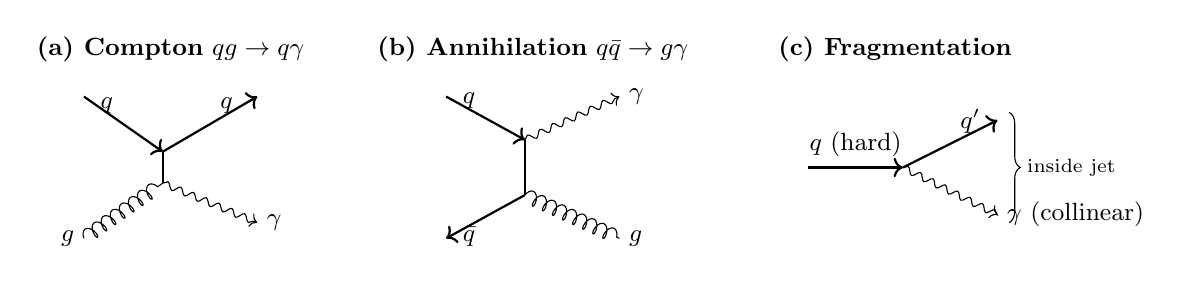
\begin{tikzpicture}[
  every node/.style={font=\small},
  photon/.style={decorate, decoration={snake, amplitude=1.2pt, segment length=5pt}, ->},
  gluon/.style={decorate, decoration={coil, amplitude=2.5pt, segment length=4pt}},
  quark/.style={->, thick}
]
% ---- (a) Compton q g -> q gamma ----
\begin{scope}[xshift=0cm]
  \node at (1.1,2.6) {\textbf{(a) Compton} $qg\to q\gamma$};
  \draw[quark] (0,2) -- (1,1.3) node[midway,above left]{$q$};
  \draw[gluon] (0,0.2) -- (1,0.9);
  \node[left] at (0,0.2) {$g$};
  \draw[thick] (1,1.3) -- (1,0.9);
  \draw[quark] (1,1.3) -- (2.2,2) node[midway,above right]{$q$};
  \draw[photon] (1,0.9) -- (2.2,0.4);
  \node[right] at (2.2,0.4) {$\gamma$};
\end{scope}
% ---- (b) annihilation q qbar -> g gamma ----
\begin{scope}[xshift=4.6cm]
  \node at (1.1,2.6) {\textbf{(b) Annihilation} $q\bar q\to g\gamma$};
  \draw[quark] (0,2) -- (1,1.45) node[midway,above left]{$q$};
  \draw[quark] (1,0.75) -- (0,0.2) node[midway,below left]{$\bar q$};
  \draw[thick] (1,1.45) -- (1,0.75);
  \draw[photon] (1,1.45) -- (2.2,2);
  \node[right] at (2.2,2) {$\gamma$};
  \draw[gluon] (1,0.75) -- (2.2,0.2);
  \node[right] at (2.2,0.2) {$g$};
\end{scope}
% ---- (c) fragmentation ----
\begin{scope}[xshift=9.2cm]
  \node at (1.1,2.6) {\textbf{(c) Fragmentation}};
  \draw[quark] (0,1.1) -- (1.2,1.1) node[midway,above]{$q$ (hard)};
  \draw[quark] (1.2,1.1) -- (2.4,1.7) node[midway,above right]{$q'$};
  \draw[photon] (1.2,1.1) -- (2.4,0.5);
  \node[right] at (2.4,0.5) {$\gamma$ (collinear)};
  \draw[decorate,decoration={brace,amplitude=4pt}] (2.55,1.8) -- (2.55,0.4)
        node[midway,right=3pt]{\scriptsize inside jet};
\end{scope}
\end{tikzpicture}
\caption{Schematic LO mechanisms (redrawn after Fig.~1 of the note). (a) and (b) make
\emph{direct} photons; (c) makes \emph{fragmentation} photons that accompany a jet. At NLO,
direct production also receives bremsstrahlung corrections.}
\end{figure}

\subsection{Why physicists care}

\begin{bgbox}
\textbf{Background: what makes photons special.} Once a photon is created in the hard scattering
it does not feel the strong force, so it escapes the collision \emph{unmodified}. That makes prompt
photons a ``clean'' probe: their production rate is computable in perturbative QCD (pQCD) without
the messy hadronization that complicates jets or hadrons.
\end{bgbox}

\begin{enumerate}[leftmargin=1.6em]
  \item \textbf{A stringent test of pQCD.} The cross section can be computed at next-to-leading
  order (NLO). Comparing data to theory tests our understanding of the strong interaction.
  \item \textbf{Direct sensitivity to the gluon PDF.} In this kinematic range the
  Compton process $qg\to q\gamma$ \emph{dominates}, so the rate is directly proportional to the
  gluon parton distribution function (PDF) of the proton. RHIC's $\roots=200$~GeV probes the
  gluon at parton momentum fractions
  \[
    x \;\sim\; \frac{2\,\ETg}{\roots} \;\approx\; 0.1\text{--}0.3 ,
  \]
  a \emph{higher-$x$} window than the LHC reaches --- so the two machines are complementary.
  \item \textbf{A reference for heavy-ion physics.} The $\pp$ result is the baseline against
  which future sPHENIX measurements in Au+Au (where photons probe the quark--gluon plasma) will
  be normalized.
  \item \textbf{Continuity with PHENIX.} It connects directly to the earlier PHENIX
  direct-photon measurement at the same energy.
\end{enumerate}

\subsection{The isolation idea}

Fragmentation photons live inside jets, so they are surrounded by other particles. Direct photons
are ``lonely.'' We exploit this with an \textbf{isolation} requirement: we sum the transverse
energy of everything within a cone of radius $\dR=\sqrt{\Delta\eta^2+\Delta\phi^2}=0.3$ around the
photon (excluding the photon itself) and demand it be small. At truth level the fiducial definition is
\[
  \boxed{\;\Eisotruth < 4~\text{GeV} \quad\text{in a cone } \dR = 0.3\;}
\]
The note shows (its Fig.~2--3) that at a 4~GeV threshold, \emph{direct} photons stay essentially
100\% efficient while \emph{fragmentation} photons are strongly suppressed. Isolation also rejects
the dominant background --- $\pi^0/\eta$ decays inside jets.

\begin{bgbox}
\textbf{Definitions you will need.}
$\ETg$ = photon transverse energy. $\eta=-\ln\tan(\theta/2)$ = pseudorapidity (0 = perpendicular
to the beam). $\phi$ = azimuth. ``Truth level'' = the generator's perfect particle list (what
really happened); ``reco level'' = what the detector reconstructs. A central theme of this note is
carefully converting reco $\to$ truth.
\end{bgbox}

% ===============================================================
\section{The detector and the data}
% ===============================================================

\subsection{The sPHENIX calorimeters in one minute}

\begin{figure}[h]
\centering
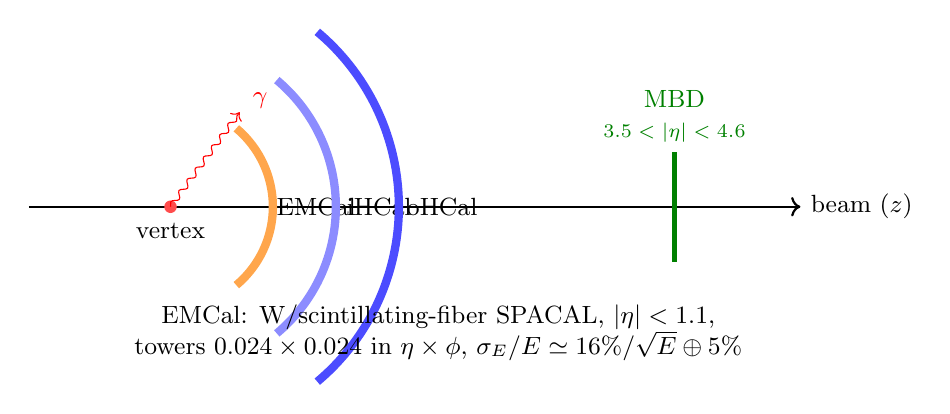
\begin{tikzpicture}[font=\small]
  % beam pipe
  \draw[->,thick] (-0.6,0) -- (9.2,0) node[right]{beam ($z$)};
  \node[circle,fill=red!70,inner sep=1.6pt,label=below:{vertex}] (v) at (1.2,0) {};
  % concentric arcs representing detector layers
  \foreach \r/\name/\col in {1.3/EMCal/orange!70, 2.1/iHCal/blue!45, 2.9/oHCal/blue!70} {
    \draw[\col, line width=3pt] (1.2,0) ++(-50:\r) arc (-50:50:\r);
    \node[black] at ($(1.2,0)+(0:\r)+(0.55,0)$) {\name};
  }
  % a photon
  \draw[decorate,decoration={snake,amplitude=1pt,segment length=5pt},->,red] (1.2,0) -- (30:2.4);
  \node[red] at (30:2.7) {$\gamma$};
  % MBD forward
  \draw[green!50!black,line width=2pt] (7.6,-0.7) -- (7.6,0.7);
  \node[green!50!black,align=center] at (7.6,1.15) {MBD\\ \scriptsize $3.5<|\eta|<4.6$};
  \node[align=center] at (4.6,-1.6) {EMCal: W/scintillating-fiber SPACAL, $|\eta|<1.1$,\\
        towers $0.024\times0.024$ in $\eta\times\phi$,
        $\sigma_E/E\simeq 16\%/\sqrt{E}\oplus 5\%$};
\end{tikzpicture}
\caption{Schematic of the relevant sPHENIX subsystems (not to scale). The EMCal measures the
photon energy; the two HCal layers contain hadronic showers and contribute to isolation; the
forward MBD provides the trigger and the collision vertex.}
\end{figure}

\begin{itemize}[leftmargin=1.4em]
  \item \textbf{EMCal} (electromagnetic calorimeter): a tungsten / scintillating-fiber SPACAL
  detector, full $2\pi$ in azimuth, $|\eta|<1.1$, finely segmented into $96\times256$ towers
  ($\Delta\eta\times\Delta\phi\approx0.024\times0.024$). Single-photon resolution
  $\sigma_E/E\simeq 16\%/\sqrt{E[\mathrm{GeV}]}\oplus 5\%$. \emph{This is where photons are
  measured.}
  \item \textbf{iHCal + oHCal} (inner/outer hadron calorimeters): sit behind the EMCal; catch
  hadronic energy and feed the isolation sum.
  \item \textbf{MBD} (Minimum Bias Detector): two arrays of 64 quartz-Cherenkov PMTs at
  $3.5<|\eta|<4.6$. Provides the minimum-bias trigger and reconstructs the collision vertex $z$.
\end{itemize}

\subsection{Data and Monte Carlo}

\begin{itemize}[leftmargin=1.4em]
  \item \textbf{Data}: Run-24 $\pp$ at $\roots=200$~GeV, runs 47289--53880, integrated
  luminosity $\mathcal{L}=64.37$~pb$^{-1}$ (production \texttt{ana521}). Selected from a
  centrally produced calorimeter ``golden run'' list with basic quality cuts.
  \item \textbf{MC}: \textsc{pythia}-8 (Detroit tune) hard-QCD + prompt-photon events passed
  through \textsc{geant}-4 with the full sPHENIX geometry. ``Photon'' samples (signal-enriched)
  and ``jet'' samples (background) are generated at several minimum-$\pT$ thresholds (5/10/20~GeV
  for photons; 8/12/20/30/40~GeV for jets) to keep statistics high at large $\pT$.
\end{itemize}

\begin{bgbox}
\textbf{Background: why stitch several MC samples together?} The cross section falls steeply with
$\pT$, so a single sample either has too few high-$\pT$ events or wastes effort at low $\pT$. Each
$\hat p_{\mathrm{T,min}}$ sample is weighted by an \emph{effective cross section}
\[
  \sigma_{\mathrm{eff}} \;=\; \sigma_{\mathrm{generator}}\,
    \frac{N_{\mathrm{accepted}}}{N_{\mathrm{generated}}},
\]
and the samples are then ``tiled'' in non-overlapping truth-leading-$\pT$ windows so the combined
spectrum is smooth across sample boundaries.
\end{bgbox}

\subsection{Pileup: ``double interactions''}

At RHIC two separate $\pp$ collisions can occur in the same bunch crossing (\textbf{pileup}, here
called a \textbf{double interaction}, DI). The MBD then reconstructs a \emph{single} vertex at the
average of the two collision points, which distorts the inferred photon $\eta$ and the shower
shapes. To handle this honestly, a set of full-\textsc{geant} \emph{DI MC} samples (two overlapping
collisions) is blended with the single-interaction (SI) samples. The data split into two
crossing-angle periods:

\begin{table}[h]
\centering
\caption{The two running periods (see Sec.~\ref{sec:pileup} for the DI machinery).}
\begin{tabular}{lcccc}
\toprule
Period & Runs & $\mathcal{L}$ & lumi region $\sigma_z$ & cluster-weighted DI \\
\midrule
0 mrad   & 47289--51274 & 47~pb$^{-1}$ & $\simeq 54$~cm & $\sim 22.4\%$ \\
1.5 mrad & 51274--54000 & 17~pb$^{-1}$ & $\simeq 22$~cm & $\sim 7.9\%$ \\
\bottomrule
\end{tabular}
\end{table}

The 1.5~mrad crossing angle geometrically shrinks the luminous region, which reduces pileup.

\subsection{Trigger and event selection}

Events are taken with the \textbf{``Photon 4~GeV''} Level-1 trigger (a high-energy EMCal cluster in
coincidence with the MBD). The trigger efficiency is measured bin-by-bin against an unbiased
MBD-only reference,
\begin{equation}
  \varepsilon_{\mathrm{trig}}(\ET) \;=\;
  \frac{N(\text{scaled[10]}\;\&\;\text{live[Nbit]})}{N(\text{scaled[10]})},
\end{equation}
and fit with a saturating (Gumbel) curve. The trigger is essentially fully efficient
($\gtrsim 99.7\%$) above $\ETg\approx 12$~GeV, which is why the result starts there. Events must
have a reconstructed vertex $|z_{\mathrm{vtx}}^{\mathrm{MBD}}| < 60$~cm.

% ===============================================================
\section{Finding the photons (reconstruction \& identification)}
% ===============================================================

\subsection{From towers to clusters}

EMCal towers above $\sim 70$~MeV that share an edge are merged into \textbf{clusters}
(\texttt{RawClusterBuilderTemplate}), with a splitting step for overlapping showers. The cluster
energy is the tower sum; its $(\eta,\phi)$ are computed relative to the MBD vertex.

\subsection{Energy scale and resolution}

The detector response is calibrated in MC by comparing reconstructed cluster $\ET$ to the truth
photon $\ET$. In each truth-$\ET$ bin the ratio $E_{\mathrm{T}}^{\mathrm{reco}}/E_{\mathrm{T}}^{\mathrm{truth}}$
is fit with a Gaussian: the mean ($\approx 0.99$, the energy \emph{scale}) and the width
($\approx 5$--7\%, the \emph{resolution}) are both excellent. The small residual scale/resolution
effects are absorbed by unfolding (Sec.~\ref{sec:unfold}).

\subsection{The background problem}

\begin{bgbox}
\textbf{Background: what fakes a prompt photon?}
The dominant fake is a high-$\pT$ $\pi^0\to\gamma\gamma$ (or $\eta\to\gamma\gamma$): at high
momentum the two decay photons are so collinear that they merge into a \emph{single} EMCal
cluster that looks photon-like. A second class is \textbf{non-physics background} (NPB): beam-gas
or beam-halo junk that streaks across the calorimeter. Without any selection, the signal-to-
background ratio is only $\sim 15\%$ at 10~GeV, rising to $\sim 50\%$ near 30~GeV.
\end{bgbox}

We separate signal from background using \textbf{shower shapes} --- moments and energy ratios of
the towers in a cluster. A genuine single photon makes a narrow, symmetric shower with most energy
in the central tower; a merged $\pi^0$ is broader or more lopsided. Key variables include:

\begin{table}[h]
\centering
\caption{The most important shower-shape variables (selected from the note's Table~4).}
\begin{tabular}{ll}
\toprule
Symbol & Meaning \\
\midrule
$E_{1\times1}/E$ & central-tower energy fraction (peaked for photons) \\
$w_\eta^{\mathrm{COGX}},\,w_\phi^{\mathrm{COGX}}$ & energy-weighted second moments (shower width) in $\eta,\phi$ \\
$E_{3\times2}/E_{3\times5}$ & energy in a $3\times2$ vs.\ $3\times5$ tower window \\
$R_{\mathrm{had}}$ & $E_{\mathrm{T}}^{\mathrm{HCal}}/(E_{\mathrm{T}}^{\mathrm{EMCal}}+E_{\mathrm{T}}^{\mathrm{HCal}})$ (hadronic leakage) \\
$\mathrm{Et1}\!-\!\mathrm{Et4}$ & energies/asymmetries of the central $2\times2$ tower block \\
\bottomrule
\end{tabular}
\end{table}

\subsection{Killing the beam junk (the NPB BDT)}

NPB clusters are spread out in $\eta$ (large $w_\eta^{\mathrm{COGX}}$) and arrive at anomalous times
relative to the MBD. A first cut $w_\eta^{\mathrm{COGX}}>1.0$ removes the worst streaks; the rest is
handled by an \textbf{XGBoost boosted decision tree (BDT)} trained to separate real collision
clusters (from MC) from streak clusters (tagged in data by anomalous timing
$t_{\mathrm{cluster}}-t_{\mathrm{MBD}}<-7$~ns). The BDT uses 25 features (note: \emph{not} timing,
so timing stays available as an independent validation). The purity is measured with a data-driven
template fit using the cluster--MBD time tail. The nominal cut $\mathrm{NPB}>0.5$ gives
$\sim99\%$ purity while keeping $\sim99\%$ of real clusters.

\subsection{Picking out photons (the photon-ID BDT)}

A \emph{second} XGBoost BDT combines 11 shower-shape features into a single photon-identification
discriminant. Clusters first pass a rectangular \textbf{pre-selection}
($E_{1\times1}/E_{3\times3}<0.98$, $0.6<\mathrm{Et1}<1.0$, $0.8<E_{3\times2}/E_{3\times5}<1.0$,
$\mathrm{NPB}>0.5$). Then:

\begin{itemize}[leftmargin=1.4em]
  \item \textbf{Tight} = pre-selection + high BDT score ($> 0.8156 - 0.00156\,\ETg$): signal-rich.
  \item \textbf{Non-tight} = pre-selection + an intermediate BDT band: background-rich
  \emph{control sample}.
\end{itemize}

\begin{bgbox}
\textbf{Why both tight and non-tight?} The non-tight sample is not garbage to be discarded --- it
is a \emph{model of the background}. The whole purity measurement (next section) relies on having a
background-enriched control region whose isolation behaviour mimics the background hiding inside the
tight signal region.
\end{bgbox}

\subsection{The isolation variable in the detector}

At reco level the analysis sums \emph{topological clusters} (a seed-and-grow calorimeter clustering,
the same scheme as ATLAS) inside a $\dR=0.4$ cone, subtracting the photon's own energy:
\[
  \Eiso = \sum_{\text{topo-clusters in cone}} \ET \;-\; E_{\mathrm{T}}^{\gamma}.
\]
Five candidate definitions were compared with ROC curves; the topo-cluster $R=0.4$ definition won
because it is robust against the EMCal noise that drifts upward over the run period (a fixed
per-tower threshold sum drifts; topo-clustering does not). The cut is set to $80\%$ signal
efficiency:
\[
  \Eiso < 0.490 + 0.0370\,E_{\mathrm{T}}^{\mathrm{reco}}\ [\text{GeV}].
\]
Note the reco isolation uses $R=0.4$ for detector performance, while the \emph{fiducial} cross
section is defined with the truth $R=0.3$, $\Eisotruth<4$~GeV cut (matching \textsc{jetphox}); the
isolation \emph{efficiency} converts between the two.

% ===============================================================
\section{Extracting the cross section (analysis procedure)}
% ===============================================================

\subsection{The workflow at a glance}

\begin{figure}[h]
\centering
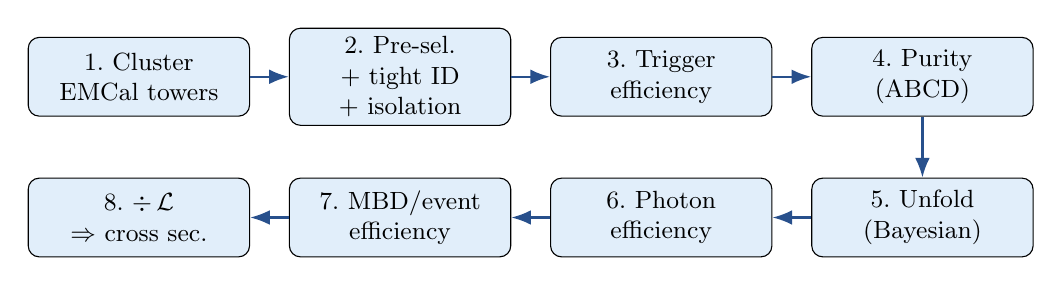
\begin{tikzpicture}[
  node distance=6pt and 14pt, font=\small,
  procstep/.style={draw, rounded corners, fill=boxblue, align=center,
               text width=2.6cm, minimum height=1.0cm, inner sep=3pt},
  arr/.style={-{Latex[length=2.5mm]}, thick, rulecol}
]
\node[procstep] (cl) {1.\ Cluster\\ EMCal towers};
\node[procstep,right=of cl] (id) {2.\ Pre-sel.\ + tight ID\\ + isolation};
\node[procstep,right=of id] (trig) {3.\ Trigger\\ efficiency};
\node[procstep,right=of trig] (pur) {4.\ Purity\\ (ABCD)};
\node[procstep,below=22pt of pur] (unf) {5.\ Unfold\\ (Bayesian)};
\node[procstep,left=of unf] (eff) {6.\ Photon\\ efficiency};
\node[procstep,left=of eff] (mbd) {7.\ MBD/event\\ efficiency};
\node[procstep,left=of mbd] (lum) {8.\ $\div\,\mathcal{L}$\\ $\Rightarrow$ cross sec.};
\draw[arr] (cl) -- (id);
\draw[arr] (id) -- (trig);
\draw[arr] (trig) -- (pur);
\draw[arr] (pur) -- (unf);
\draw[arr] (unf) -- (eff);
\draw[arr] (eff) -- (mbd);
\draw[arr] (mbd) -- (lum);
\end{tikzpicture}
\caption{The eight-step analysis chain. Each box is unpacked in the text below.}
\end{figure}

\subsection{Purity: the ABCD (double-sideband) method}
\label{sec:abcd}

Even after tight ID + isolation, some background survives. We must measure the
\textbf{purity} $P$ = (signal fraction in the signal region) and correct for it. This is done
\emph{from data}, using the assumption that the photon-ID and isolation discriminants are
approximately \textbf{independent} for background.

\begin{figure}[h]
\centering
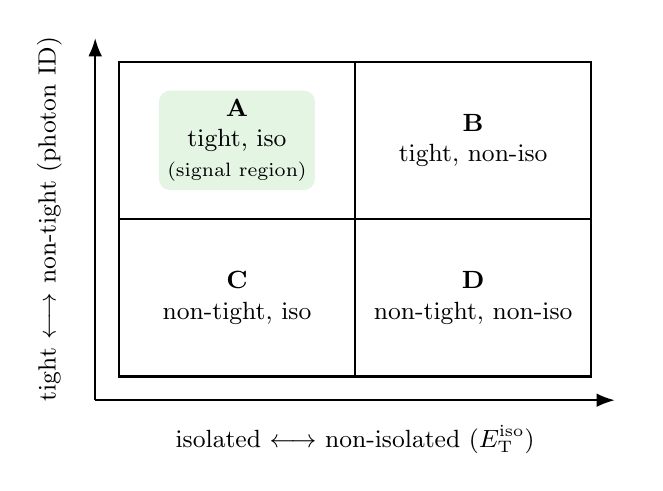
\begin{tikzpicture}[font=\small]
  \draw[thick] (0,0) rectangle (6,4);
  \draw[thick] (3,0) -- (3,4);
  \draw[thick] (0,2) -- (6,2);
  % labels
  \node[align=center,fill=boxgreen,rounded corners,inner sep=3pt] at (1.5,3) {\textbf{A}\\ tight,\ iso\\ \scriptsize(signal region)};
  \node[align=center] at (4.5,3) {\textbf{B}\\ tight,\ non-iso};
  \node[align=center] at (1.5,1) {\textbf{C}\\ non-tight,\ iso};
  \node[align=center] at (4.5,1) {\textbf{D}\\ non-tight,\ non-iso};
  % axes
  \draw[-{Latex},thick] (-0.3,-0.3) -- (6.3,-0.3) node[right]{};
  \node[below] at (3,-0.5) {isolated $\longleftrightarrow$ non-isolated ($\Eiso$)};
  \draw[-{Latex},thick] (-0.3,-0.3) -- (-0.3,4.3);
  \node[rotate=90,above] at (-0.6,2) {tight $\longleftrightarrow$ non-tight (photon ID)};
\end{tikzpicture}
\caption{The ABCD method (redrawn after the note's Fig.~26). Region A is the signal region.
If isolation and ID are independent for background, the background in A can be predicted from the
three control regions B, C, D.}
\end{figure}

If background ID and isolation are uncorrelated, then $N_A^{\mathrm{bkg}}/N_B^{\mathrm{bkg}}
= N_C^{\mathrm{bkg}}/N_D^{\mathrm{bkg}}$, which lets us \emph{predict} the background in A from the
sidebands. The number of signal clusters in A is
\begin{equation}
  N^{A,\mathrm{data}}_{\mathrm{signal}} \;=\;
  N^{A,\mathrm{data}}_{\mathrm{raw}} - \frac{N^{B,\mathrm{data}}_{\mathrm{raw}}\,
  N^{C,\mathrm{data}}_{\mathrm{raw}}}{N^{D,\mathrm{data}}_{\mathrm{raw}}}.
\end{equation}
A real subtlety: \emph{signal} photons also leak into the control regions B, C, D. This is corrected
using signal-MC leakage fractions $f^{X,\mathrm{MC}}=N^{X,\mathrm{MC}}_{\mathrm{signal}}/N^{A,\mathrm{MC}}_{\mathrm{signal}}$,
giving the leakage-corrected equation (the note's Eq.~4). The purity is then
\begin{equation}
  P \;=\; \frac{N^A_{\mathrm{signal}}}{N^A}.
\end{equation}
The measured purity (leakage-corrected) rises with $\ETg$:
\[
  P \approx 0.51 \;(10\text{--}12~\text{GeV}) \;\to\; 0.72 \;(18\text{--}20~\text{GeV})
    \;\to\; 0.90 \;(>26~\text{GeV}),
\]
exactly as expected since the $\pi^0$ background falls faster than the signal.

\begin{bgbox}
\textbf{Background: ``the ABCD method'' is a workhorse of HEP.} It lets you measure a background
\emph{from data} using two (nearly) independent variables, instead of trusting the MC normalization.
The price is the independence assumption; the residual correlation here is measured in MC (the
``closure correction'' $C_{\mathrm{MC}}=P^{\mathrm{MC}}_{\mathrm{truth}}/P^{\mathrm{MC}}_{\mathrm{ABCD}}$)
and propagated as a \emph{systematic} rather than applied as a correction --- the same conservative
choice ATLAS makes.
\end{bgbox}

\subsection{Efficiency}

The chain of efficiencies, all vs.\ truth $\ETg$, accounts for everything we lose:
\textbf{reconstruction} (truth photon $\to$ matched cluster), \textbf{identification} (passes
tight ID), \textbf{isolation} (passes iso cut), and the \textbf{MBD vertex} efficiency (event has
an N--S coincidence and a reconstructed vertex in $|z|<60$~cm). Truth--reco matching uses the
\textsc{geant} track-ID via \texttt{CaloRawClusterEval}. Each is applied as a bin-by-bin
correction after unfolding.

\subsection{Unfolding}
\label{sec:unfold}

\begin{bgbox}
\textbf{Background: what is unfolding and why do it?} The detector smears the true $\ETg$ spectrum
(finite resolution + bin migration). \emph{Unfolding} inverts this smearing to recover the true
spectrum, so the result can be compared to theory or other experiments without anyone needing the
sPHENIX detector simulation. The relationship is $\vec{y}_{\mathrm{reco}} = R\,\vec{x}_{\mathrm{truth}}$,
where $R$ is the \emph{response matrix}; unfolding estimates $\vec{x}$ from $\vec{y}$.
\end{bgbox}

The note uses the \textbf{D'Agostini iterative Bayesian} method (\texttt{RooUnfold}). Because the
EMCal resolution is excellent, $R$ is nearly diagonal and unfolding barely moves the spectrum
(2--10\% effect). The MC prior is reweighted to match the data shape (a Pad\'e fit of the
data/MC ratio), and the number of iterations is set to $N_{\mathrm{iter}}=2$ --- the point where
iteration-to-iteration changes drop below the statistical error. \textbf{Closure tests} (unfold the
MC with a matrix built from the same or an independent half of the MC) reproduce the truth spectrum
to within $\sim2\%$.

\subsection{Luminosity}

The integrated luminosity $\mathcal{L}=64.37$~pb$^{-1}$ is the beam-delivered value sampled by the
Photon-4-GeV trigger, computed from the live MBD coincidence rate divided by the trigger prescale
and the calibrated MBD inelastic cross section
$\sigma_{\mathrm{MBD}}=25.2^{+2.3}_{-1.7}$~mb (measured in a dedicated van-der-Meer scan). The
$\sigma_{\mathrm{MBD}}$ uncertainty gives the asymmetric luminosity systematic
$+9.13\%/-6.75\%$.

% ===============================================================
\section{Systematic uncertainties}
% ===============================================================

Every systematic is evaluated by \emph{rerunning the whole analysis} with one ingredient varied and
taking the per-bin change in the cross section. The contributions are added in quadrature per
$\ETg$ bin. Table~\ref{tab:syst} lists the maximum size of each source.

\begin{table}[h]
\centering
\caption{Maximum per-bin systematic by source over $12<\ETg<32$~GeV (from the note's Table~7).
``low/high'' are the down/up variations.}
\label{tab:syst}
\begin{tabular}{lcc}
\toprule
Source & low max [\%] & high max [\%] \\
\midrule
Energy scale (flat $\pm1.1\%$)     & 10.5 & 11.9 \\
Energy scale (non-linearity)       & 7.3  & 7.3  \\
\textbf{Energy resolution}         & \textbf{21.2} & \textbf{21.2} \\
Purity -- tight ID                 & 6.7  & 6.7  \\
Purity -- non-tight ID             & 2.4  & 2.4  \\
Purity -- non-isolation gap        & 3.8  & 1.0  \\
Purity -- fit functional form      & 0.3  & 0.3  \\
Purity -- fit statistics (1$\sigma$)& 4.4 & 4.4  \\
Purity -- MC closure correction    & 5.8  & 5.8  \\
Efficiency -- $\Eiso$ shape        & 4.7  & 4.7  \\
Efficiency -- generator (\textsc{herwig}) & 5.8 & 5.8 \\
MBD vertex efficiency              & 6.0  & 6.0  \\
Unfolding -- response reweight     & 0.4  & 0.4  \\
Unfolding -- iteration scan        & 5.5  & 5.5  \\
Double-interaction                 & 1.6  & 1.6  \\
Non-physics-background cut         & 1.0  & 4.5  \\
Luminosity (flat)                  & 6.8  & 9.1  \\
\midrule
\textbf{Total (per-bin)}           & \textbf{30.8} & \textbf{31.7} \\
\bottomrule
\end{tabular}
\end{table}

\begin{bgbox}
\textbf{Reading the table.} The budget is dominated by the \textbf{energy scale} and
\textbf{resolution}. The reason is the steeply falling spectrum: a tiny shift in measured energy
moves many events between bins, and because there are far more low-$\ETg$ events than high-$\ETg$
ones, even a $\sim1\%$ energy mis-scale produces a large \emph{migration} effect at high $\ETg$.
The purity (fit-CI and MC-closure) and luminosity drive the \emph{low}-$\ETg$ budget. The per-bin
maxima occur in different bins, so the column sums are \emph{not} the total --- the meaningful
quantity is the per-bin quadrature, which reaches $\approx -31\%/+32\%$ at the high-$\ETg$ end.
\end{bgbox}

% ===============================================================
\section{Results}
% ===============================================================

The differential cross section is built as
\begin{align}
  Y_{\mathrm{rec}}(\ETg) &= \mathrm{Unfold}\!\left[\,N^{\gamma}_{\mathrm{tight,iso}}(\ETg)\times P(\ETg)\,\right],\\[3pt]
  \frac{d\sigma}{d\ETg\,d\eta^\gamma} &= \frac{1}{\mathcal{L}}\,
     \frac{Y_{\mathrm{rec}}}{\mathcal{E}}\,\frac{1}{\Delta\ETg\,\Delta\eta^\gamma}.
\end{align}
That is: raw tight+isolated yield $\to$ multiply by purity $\to$ unfold $\to$ divide by efficiency
$\to$ divide by luminosity and bin widths.

\begin{nutshell}
\textbf{The headline result.} Over $12<\ETg<32$~GeV the measured isolated-prompt-photon cross
section falls by roughly two orders of magnitude and \textbf{agrees within experimental
uncertainties} with:
\begin{itemize}[leftmargin=1.4em,topsep=2pt,itemsep=1pt]
  \item \textbf{NLO pQCD} from \textsc{jetphox} (v1.3.1.4; CT14nlo PDF, BFG~II fragmentation
  functions, scales $\mu_R=\mu_F=\mu_f=\ETg$),
  \item \textbf{\textsc{pythia}-8} (v8.307, Detroit tune),
  \item the previous \textbf{PHENIX} direct-photon measurement at the same $\roots=200$~GeV
  (after correcting for PHENIX's different rapidity window and bin definition).
\end{itemize}
Systematics dominate the uncertainty across the range; statistical errors grow from sub-percent at
low $\ETg$ to $\sim30\%$ in the highest bin but stay subdominant.
\end{nutshell}

\begin{bgbox}
\textbf{What the agreement \emph{means}.} Because the Compton process dominates here, agreement
with NLO pQCD confirms that the proton's \textbf{gluon PDF} at $x\sim0.1$--$0.3$ is well described,
and validates sPHENIX's photon reconstruction as a tool for the upcoming heavy-ion program. The
consistency with PHENIX (whose points carry \emph{no} isolation requirement) is itself evidence
that the fragmentation contribution left after the $\Eisotruth<4$~GeV cut is small --- exactly the
gluon--Compton-dominance picture.
\end{bgbox}

\subsection{Comparison to PHENIX (an instructive cross-check)}

PHENIX reported \emph{inclusive} direct photons in $|\eta|<0.25$ as $d\sigma/(d\eta\,d\ETg)$. To
overlay it fairly on the sPHENIX $|\eta|<0.7$ isolated measurement, two corrections are applied:
\begin{enumerate}[leftmargin=1.6em]
  \item \textbf{Bin-width recovery}: a smooth modified-power-law fit removes the few-percent
  distortion of plotting a steeply falling spectrum at the bin centre.
  \item \textbf{Pseudorapidity-density rescaling}: the ratio
  $R(\ETg)=(dN/d\eta)_{|\eta|<0.25}/(dN/d\eta)_{|\eta|<0.7}$ from truth MC. It is $\approx1$
  below 14~GeV and rises to $\approx1.22$ at the highest $\ETg$, because higher-$x$ production
  is more central in rapidity.
\end{enumerate}
After these, the corrected PHENIX spectrum agrees with sPHENIX across the overlap.

% ===============================================================
\section{Selected deep-dives (the appendices, distilled)}
% ===============================================================

The note's appendices are cross-checks that build confidence in the result. The most physically
interesting ones:

\subsection{Double-interaction (pileup) physics}
\label{sec:pileup}

\begin{figure}[h]
\centering
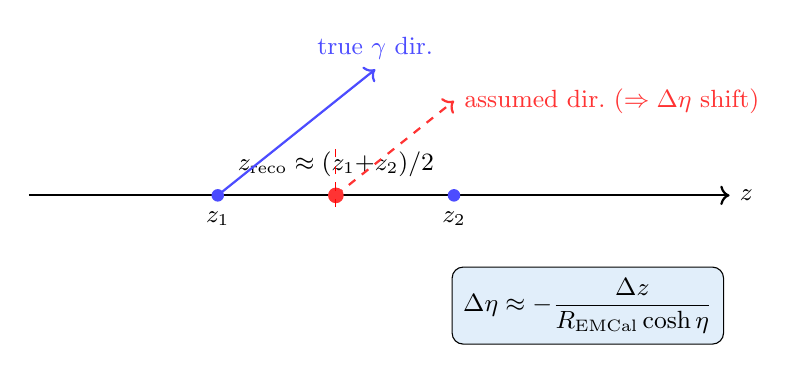
\begin{tikzpicture}[font=\small]
  \draw[->,thick] (-0.4,0) -- (8.5,0) node[right]{$z$};
  % truth vertices
  \node[circle,fill=blue!70,inner sep=1.6pt,label=below:{$z_1$}] (z1) at (2.0,0) {};
  \node[circle,fill=blue!70,inner sep=1.6pt,label=below:{$z_2$}] (z2) at (5.0,0) {};
  % reco vertex
  \node[circle,fill=red!80,inner sep=2pt,label=above:{$z_{\mathrm{reco}}\approx(z_1{+}z_2)/2$}] (zr) at (3.5,0) {};
  \draw[red,dashed] (3.5,-0.15) -- (3.5,0.6);
  % photon true direction from z1 vs assumed from zreco
  \draw[->,blue!70,thick] (2.0,0) -- (4.0,1.6) node[above]{true $\gamma$ dir.};
  \draw[->,red!80,thick,dashed] (3.5,0) -- (5.0,1.2) node[right]{assumed dir.\ ($\Rightarrow \Delta\eta$ shift)};
  \node[align=left,draw,rounded corners,fill=boxblue,inner sep=4pt] at (6.7,-1.4)
       {$\displaystyle \Delta\eta \approx -\frac{\Delta z}{R_{\mathrm{EMCal}}\cosh\eta}$};
\end{tikzpicture}
\caption{The vertex-shift mechanism. Two collisions at $z_1,z_2$ give one reconstructed vertex at
their average. A photon born at $z_1$ but assigned to $z_{\mathrm{reco}}$ acquires a wrong $\eta$,
which distorts its shower shapes and feeds the $\ETg$-dependent BDT threshold.}
\end{figure}

The mean number of interactions per crossing $\mu$ is derived from the MBD rate; a zero-truncated
Poisson gives the single/double fractions, converted to \emph{cluster-weighted} mixing weights
$w_{\mathrm{single}},w_{\mathrm{double}}$ (Table~\ref{tab:pileup}). The dominant DI effect is on
\textbf{reconstruction efficiency} (a $\sim20$ percentage-point drop in pure-DI MC, from cluster
loss + shifted kinematics) and on the \textbf{photon-ID BDT} (a $\sim13$~pp drop). Crucially, all
of this is absorbed \emph{automatically} because the efficiency, response matrix, and background
template are all built from the SI+DI \emph{blended} MC --- there is no separate ad-hoc DI
correction. A truth-vertex reweight (factorized $w(z_h)w(z_{\mathrm{mb}})$ for DI events) further
aligns the MC vertex distribution to data.

\begin{table}[h]
\centering
\caption{Pileup fractions and mixing weights (the note's Table~10). $f_1,f_2$ are
event-level single/double fractions; $w$ are cluster-weighted.}
\label{tab:pileup}
\begin{tabular}{lccccc}
\toprule
Crossing & $\mu_{\mathrm{corr}}$ & $f_1$ & $f_2$ & $w_{\mathrm{single}}$ & $w_{\mathrm{double}}$ \\
\midrule
0 mrad   & 0.24 & 0.879 & 0.111 & 0.776 & 0.224 \\
1.5 mrad & 0.08 & 0.960 & 0.039 & 0.921 & 0.079 \\
\bottomrule
\end{tabular}
\end{table}

\subsection{Other cross-checks worth knowing}
\begin{itemize}[leftmargin=1.4em]
  \item \textbf{Back-to-back jet test of the NPB BDT}: in a sample physically depleted of beam junk
  (require a recoil jet), turning the NPB BDT on/off changes the cross section by $\le1\%$ ---
  proving the BDT does not bias real photons.
  \item \textbf{$\phi$-symmetry dead-tower study}: because the cluster rate should be flat in
  $\phi$ at fixed $\eta$, deviations flag dead towers not modelled in MC. Masking them symmetrically
  in data and MC shifts the integrated cross section by $\sim2\%$ (assigned as an acceptance
  systematic).
  \item \textbf{\textsc{jetphox} PDF comparison}: swapping CT14nlo $\to$ CT14lo $\to$ NNPDF3.1
  shows the LO-vs-NLO gluon difference (a crossover near $\ETg\approx14$~GeV); the two NLO PDF
  families agree to within $\pm3$--20\%.
  \item \textbf{\textsc{herwig} generator cross-check}: re-running with \textsc{herwig}-7 instead
  of \textsc{pythia}-8 mainly shifts the isolation efficiency by 3--6\% (\textsc{herwig} has less
  underlying-event activity); propagated as an efficiency systematic.
\end{itemize}

% ===============================================================
\section{Glossary \& takeaways}
% ===============================================================

\begin{table}[h]
\centering
\caption{Quick-reference glossary.}
\begin{tabular}{ll}
\toprule
Term & Meaning \\
\midrule
Prompt photon & photon from the hard scatter (direct or fragmentation) \\
Direct / fragmentation $\gamma$ & from $2\to2$ vertex / radiated off a final-state quark \\
Isolation & small extra energy in a cone $\Rightarrow$ ``lonely'' photon $\Rightarrow$ signal \\
Shower shape & tower-level moments distinguishing $\gamma$ from $\pi^0/$junk \\
NPB & non-physics background (beam-gas/halo streaks) \\
BDT & boosted decision tree (multivariate classifier; XGBoost here) \\
ABCD method & data-driven background subtraction via 4 regions \\
Purity $P$ & signal fraction in the tight+isolated region \\
Unfolding & undo detector smearing to recover the true spectrum \\
DI / pileup & two $\pp$ collisions in one bunch crossing \\
PDF & parton distribution function (here, the gluon is key) \\
\bottomrule
\end{tabular}
\end{table}

\begin{nutshell}
\textbf{Three things to remember.}
(1) Prompt photons are a \emph{clean} pQCD probe and, at RHIC kinematics, a near-direct gluon-PDF
measurement at $x\sim0.1$--$0.3$.
(2) The hard part is separating real photons from $\pi^0$ decays and beam junk --- solved with
shower-shape BDTs, isolation, and the data-driven ABCD purity method.
(3) The Run-24 sPHENIX result agrees with NLO pQCD, \textsc{pythia}-8, and PHENIX, establishing
the photon channel for the heavy-ion program.
\end{nutshell}

\vspace{8pt}
\noindent\textit{Note: the official note flags its EMCal energy-scale variation ($\pm1.1\%$) as a
placeholder pending the Calorimeter Calibration group's final guidance, so the high-$\ETg$
systematic envelope may be re-evaluated.}

\vspace{12pt}
\noindent\textbf{Key references} (from the note): PHENIX direct photons, PRD~\textbf{86}, 072008
(2012); \textsc{pythia}-8, Comput.~Phys.~Commun.~\textbf{191}, 159 (2015); \textsc{geant}-4,
NIM~A~\textbf{506}, 250 (2003); D'Agostini unfolding, arXiv:1010.0632; ATLAS topo-clusters,
EPJC~\textbf{77}, 490 (2017); Detroit tune, PRD~\textbf{105}, 016011 (2022); BFG fragmentation
functions, EPJ~\textbf{2}, 529 (1998).

\end{document}
